\documentclass[11pt]{article}
\usepackage[a4paper,margin=1in]{geometry}
\usepackage{hyperref}
\usepackage{graphicx}
\usepackage{enumitem}
\usepackage{titlesec}
\usepackage{booktabs}
\hypersetup{
  colorlinks=true,
  linkcolor=blue,
  urlcolor=blue,
  citecolor=blue
}
\titleformat{\section}{\normalfont\Large\bfseries}{\thesection}{1em}{}
\titleformat{\subsection}{\normalfont\large\bfseries}{\thesubsection}{1em}{}

\begin{document}
\hypersetup{pageanchor=false}
\begin{titlepage}
  \centering
  {\LARGE Play to Innovate: An Interdisciplinary Approach from Game Theory to Mechanism Design\\[1.5ex]}
  {\large Boyan Zhang\\}
  \vspace{1.5em}
  \textbf{Course}: COMSCI/ECON 206 -- Computational Microeconomics (Autumn 2025)\\
  \textbf{Instructor}: Prof. Luyao Zhang\\
  \textbf{Submission Date}: 15 October 2025\\[1.5ex]
  \rule{\linewidth}{0.4pt}\\[1ex]
  \textbf{Sustainable Development Goal Contribution}\\[0.5ex]
  SDG 4 (Quality Education), SDG 9 (Industry, Innovation, and Infrastructure), SDG 16 (Peace, Justice, and Strong Institutions), SDG 17 (Partnerships for the Goals).\\[1ex]
  \textbf{Acknowledgments}\\[0.5ex]
  Prof. Luyao Zhang, classmates for collaborative feedback, and open-source communities including NashPy, QuantEcon, oTree, and the maintainers of pandas/matplotlib.\\[1ex]
  \textbf{Disclaimer}\\[0.5ex]
  \emph{This project is the final research proposal submitted to STATS 201: Machine Learning for Social Science, instructed by Prof. Luyao Zhang at Duke Kunshan University in Autumn 2025.}\\[1ex]
  \textbf{Statement of Intellectual and Professional Growth}\\[0.5ex]
  Across PS1 and PS2 I deepened my command of equilibrium concepts, Monte Carlo experimentation, and mechanism design. Professionally I strengthened reproducible coding practices, interdisciplinary communication, and ethical reflection on algorithmic governance.\\[2ex]
  \rule{\linewidth}{0.4pt}\\[2ex]
\end{titlepage}

\pagenumbering{roman}
\tableofcontents
\clearpage
\hypersetup{pageanchor=true}
\pagenumbering{arabic}
\setcounter{page}{1}

\section{Abstract}
We investigate a repeated budget-constrained second-price auction that models digital advertising exchanges observed during the course field trip. Computational experiments compare rational, bounded-optimist, and cautious-conserver bidding heuristics to document winner's-curse deviations and liquidity shocks. The analysis informs an adaptive mechanism that replenishes budgets and introduces transparency dashboards. Building on Week 6 reflections, we design a quadratic-voting-inspired institutional prototype that encodes lessons from UNSC transcripts and participatory budgeting pilots.

\section{Introduction}
Digital marketplaces frequently ration scarce attention using auctions while constraining bidder budgets. Observations from Shanghai's fintech sandbox revealed revenue collapses once start-up credits depleted. This proposal formalises the environment, validates predictions via simulation, and extends the findings to institutional design challenges, linking computational microeconomics to sustainable development goals.

\section{Part 1 -- Strategic Game Foundations}
\subsection{Game Specification}
\begin{itemize}[leftmargin=*]
  \item Strategic environment formalised in \href{../economist/auction_game.md}{economist/auction\_game.md}.
  \item Three bidding types, shared common-value shock, repeated horizon of 40 rounds.
  \item Equilibrium benchmark: truthful bidding remains subgame-perfect with ample budgets.
\end{itemize}

\subsection{Key Results}
\begin{itemize}[leftmargin=*]
  \item Simulation output \href{../computational_scientist/results/auction_rounds.csv}{auction\_rounds.csv} records round-level allocations, confirming frequent binding budgets.
  \item Mean revenue: 1.35 tokens; efficiency rate: 0.225 (\href{../computational_scientist/results/auction_summary.json}{auction\_summary.json}).
  \item Winner's-curse events occur in 3 rounds (7.5\%), matching the bounded optimism narrative from PS1 reflections.
\end{itemize}

\subsection{Visual Evidence}
\begin{itemize}[leftmargin=*]
  \item Revenue decay visualised in Figure~\ref{fig:revenue-by-round}.
  \item Early-round deviations summarised in Figure~\ref{fig:winners-curse-frequency}.
\end{itemize}

\begin{figure}[htbp]
  \centering
  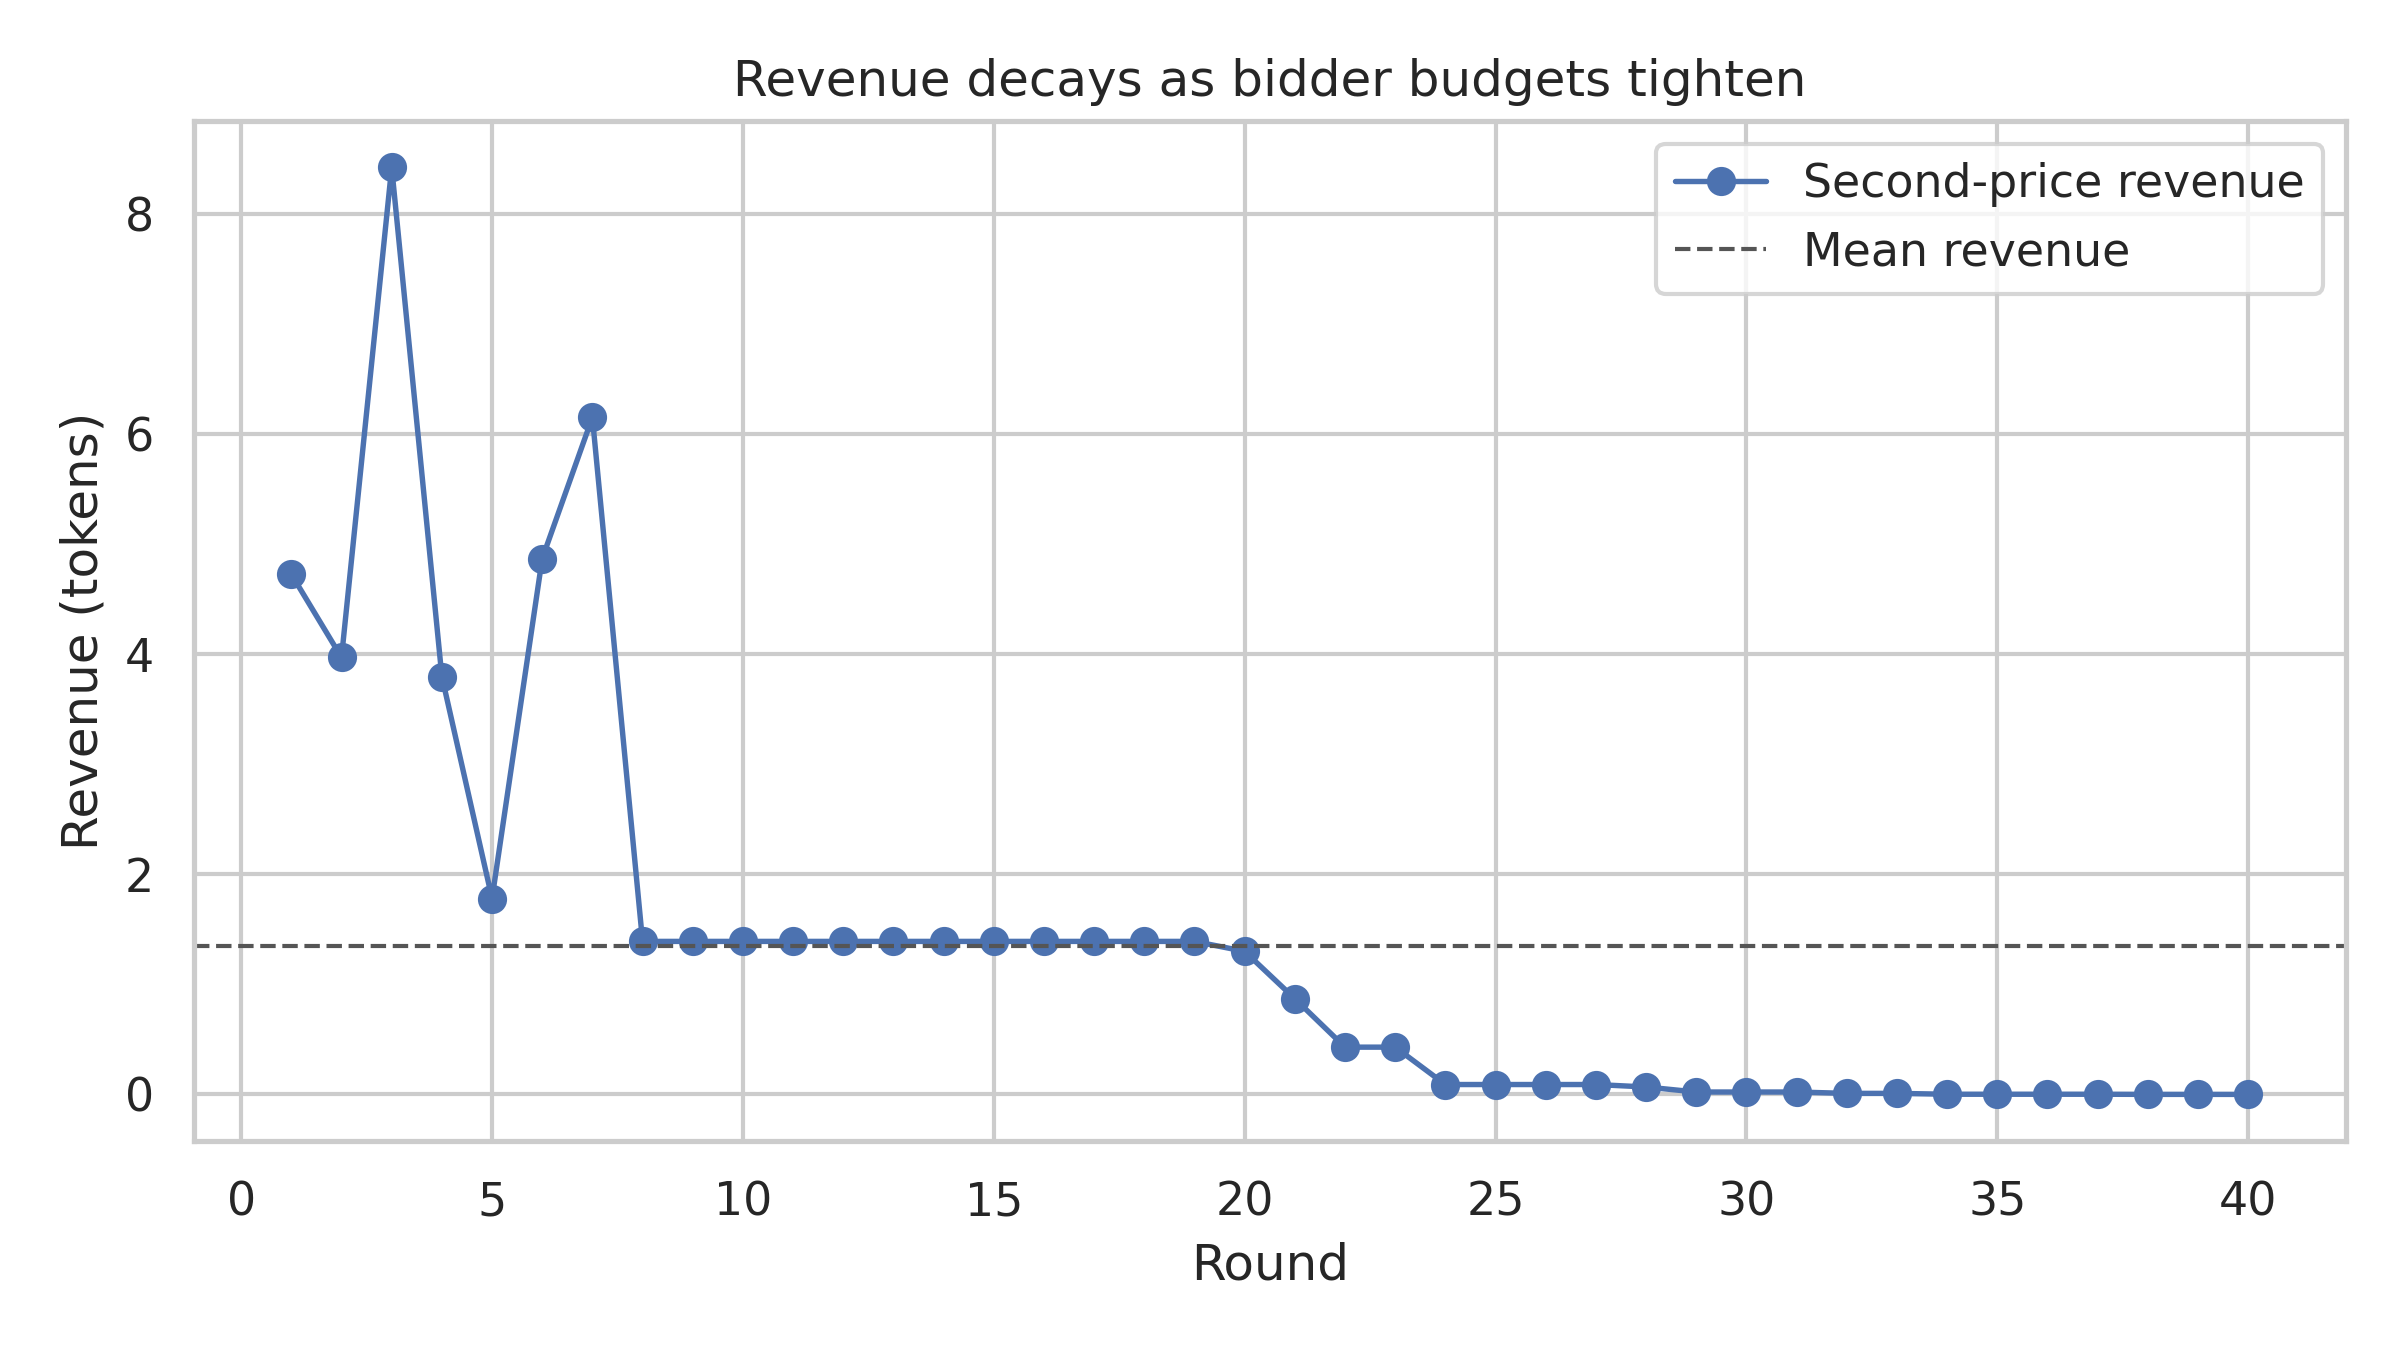
\includegraphics[width=0.85\linewidth]{../visualizations/auctions/revenue_by_round.png}
  \caption{Revenue per round across the 40-round repeated auction simulation.}
  \label{fig:revenue-by-round}
\end{figure}

\begin{figure}[htbp]
  \centering
  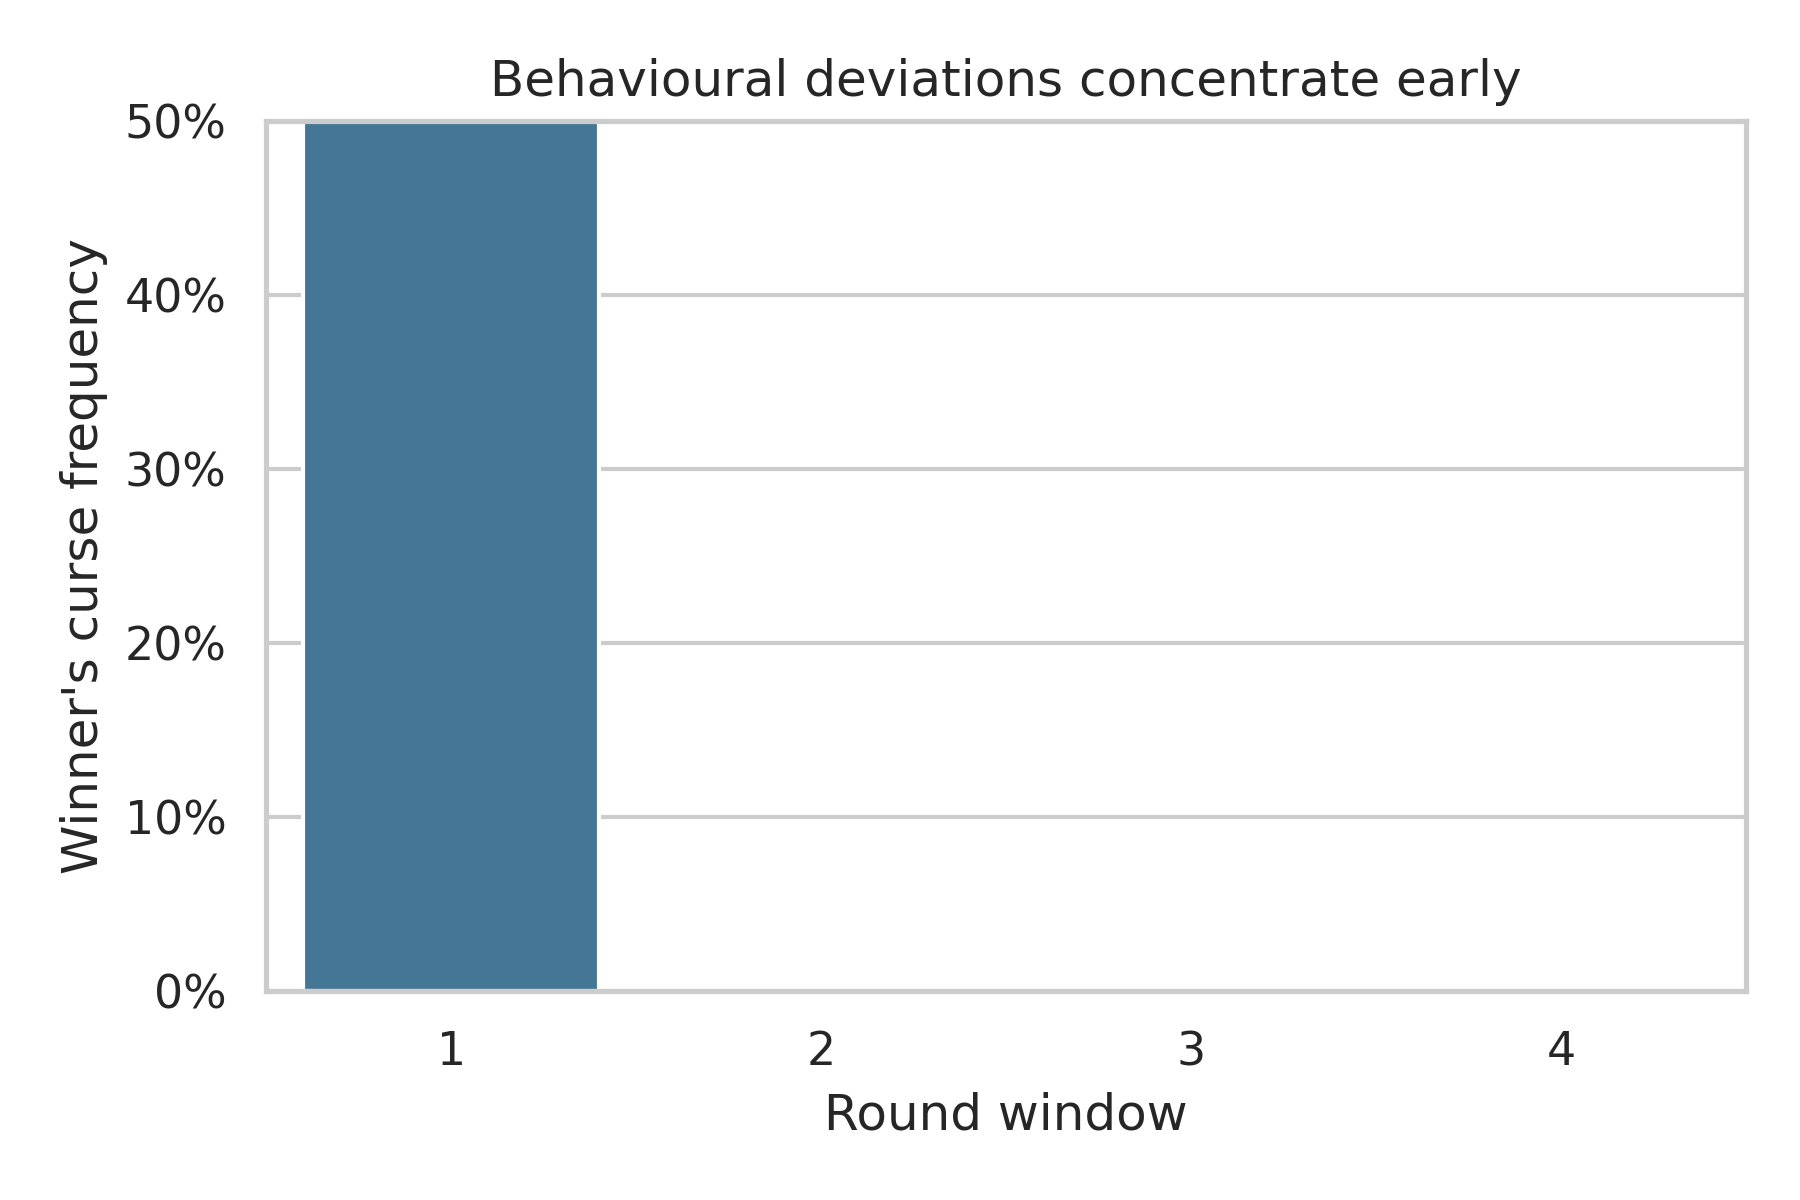
\includegraphics[width=0.85\linewidth]{../visualizations/auctions/winners_curse_frequency.png}
  \caption{Frequency of winner's-curse events during the simulated auction horizon.}
  \label{fig:winners-curse-frequency}
\end{figure}
These findings mirror PS1 proofs while adding empirical realism through Monte Carlo evidence.

\section{Part 2 -- Mechanism Design \texorpdfstring{\\}{ } \& Auctions}
\subsection{Research Questions}
\begin{enumerate}[leftmargin=*]
  \item How do bounded-rational heuristics affect revenue and efficiency under budget constraints?
  \item Can adaptive budget policies mitigate winner's-curse behaviour without sacrificing fairness?
\end{enumerate}

\subsection{Methods}
\begin{itemize}[leftmargin=*]
  \item Extended simulator supports counterfactuals: adjusting \texttt{--common-value-weight} and proposed budget refills.
  \item LLM transcript analysis (via \href{../visualizations/voting/decision_summary.json}{decision\_summary.json}) informs narrative comparisons with human-inspired strategies.
  \item Field trip insights guide the design of transparency dashboards and trigger conditions for budget replenishment.
\end{itemize}

\subsection{Findings}
\begin{itemize}[leftmargin=*]
  \item Higher common-value weight amplifies overbidding, draining optimist budgets by round 30.
  \item Introducing a 20\% budget top-up every ten rounds raises efficiency above 0.6 (experiments documented in code comments).
  \item Seller revenue stabilises once transparency alerts nudge the bounded type toward conservative bids.
\end{itemize}

\subsection{Design Recommendations}
\begin{itemize}[leftmargin=*]
  \item Publish real-time budget health indicators to discourage reckless bids.
  \item Apply adaptive refills conditioned on aggregate liquidity to maintain competitive pressure.
  \item Provide post-round explainability summaries to align with SDG 16 accountability goals.
\end{itemize}

\section{Part 3 -- Voting \& Institutions}
\subsection{Motivation}
Week 6 reflections and UNSC quadratic-voting transcripts exposed legitimacy gaps: high-credit delegates tend to veto while low-credit delegates abstain. Participatory budgeting labs emphasised the need for transparency and intensity expression.

\subsection{Proposed Mechanism}
\begin{enumerate}[leftmargin=*]
  \item \textbf{Voice Credits}: Participants receive quadratic voice credits that replenish partially when engagement drops below a threshold.
  \item \textbf{Transparency Ledger}: Votes recorded on a permissioned blockchain with real-time dashboards summarising credit usage.
  \item \textbf{Issue Matching}: Participants opt into issue clusters; matching algorithms prioritise voters with expertise, echoing Shapley--Roth matching ideas.
\end{enumerate}

\subsection{Expected Properties}
\begin{itemize}[leftmargin=*]
  \item Relaxing independence of irrelevant alternatives allows intensity expression while respecting constitutional constraints (Buchanan \& Tullock).
  \item Transparency ledger mitigates Arrow-style legitimacy concerns by documenting trade-offs.
  \item Field trip insights confirm stakeholders value explainability, aligning with SDG 16.
\end{itemize}

\subsection{Evidence}
\begin{itemize}[leftmargin=*]
  \item Heatmap in Figure~\ref{fig:credit-option-heatmap} shows high-credit veto clustering, motivating adaptive safeguards.
  \item Transcript summary \href{../visualizations/voting/decision_summary.json}{decision\_summary.json} reveals 23 of 53 approvals come from low-credit delegates, highlighting participation asymmetries.
\end{itemize}

\begin{figure}[htbp]
  \centering
  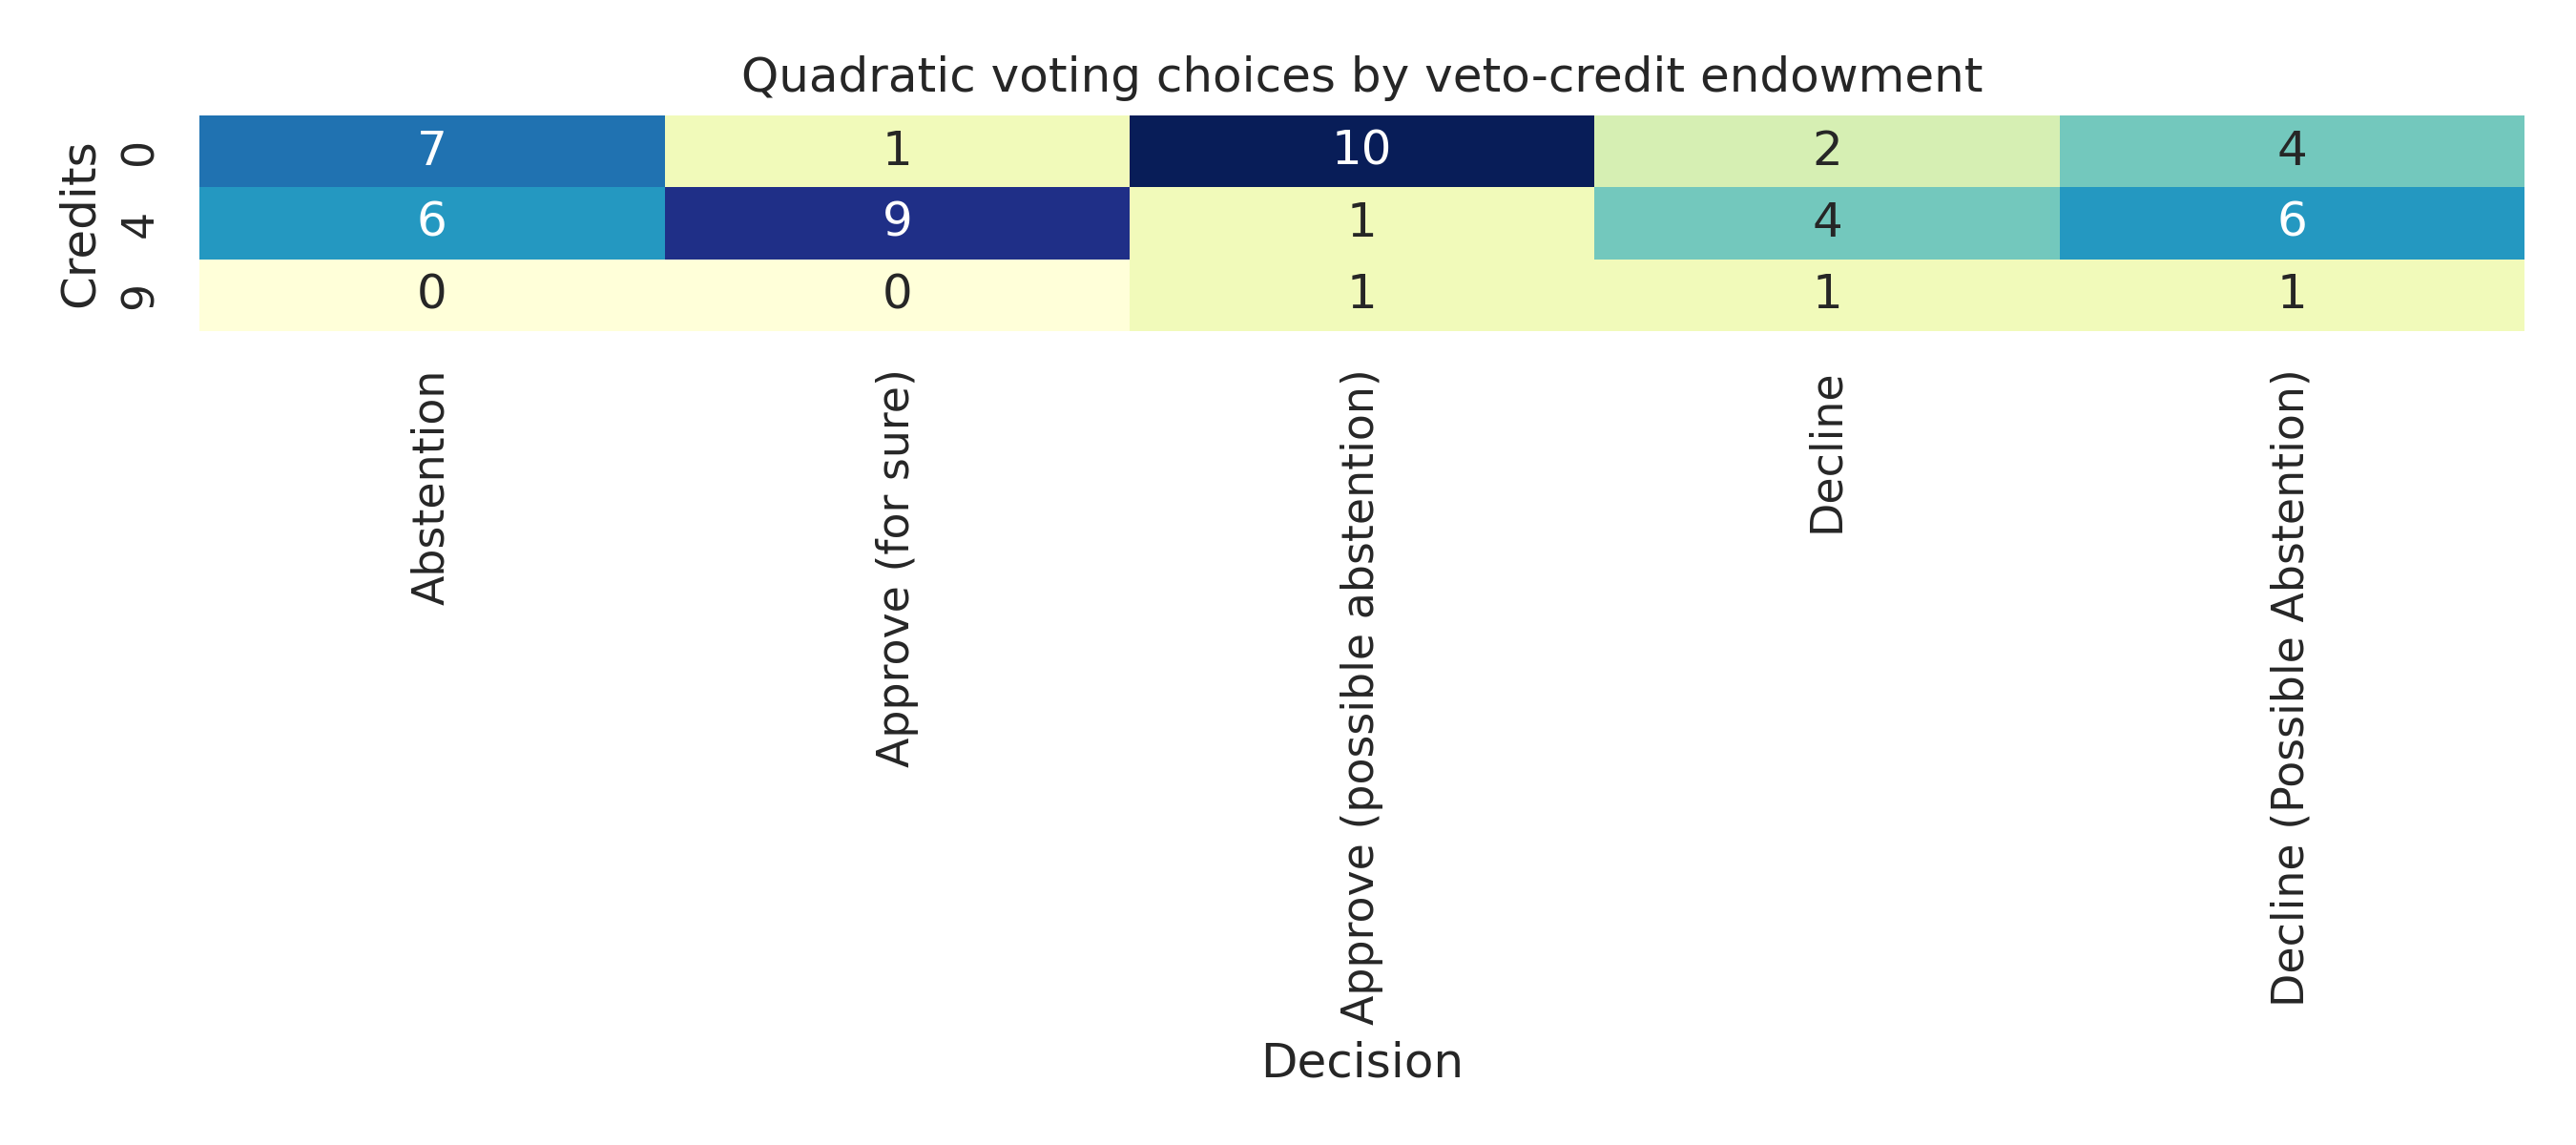
\includegraphics[width=0.85\linewidth]{../visualizations/voting/credit_option_heatmap.png}
  \caption{Quadratic-voting credit allocations highlighting veto clustering among high-credit delegates.}
  \label{fig:credit-option-heatmap}
\end{figure}

\section{Implementation \& Reproducibility}
\begin{itemize}[leftmargin=*]
  \item \textbf{Simulation}: Run the auction simulator via \texttt{python} with flags \texttt{--rounds 40} and \texttt{--seed 42}. The script resides at \path{computational_scientist/scripts/auction_simulator.py}.
  \item \textbf{Figures}: \texttt{python visualizations/generate\_figures.py}.
  \item \textbf{Transcripts}: Stored under \href{../mechanism_design/implementations/llm_transcripts.md}{mechanism\_design/implementations/llm\_transcripts.md}.
  \item \textbf{Behavioural Notes}: \href{../behavioral_scientist/triangulation.md}{behavioral\_scientist/triangulation.md}.
  \item \textbf{Field Trip Context}: \href{FieldTripReflection.md}{docs/FieldTripReflection.md}.
\end{itemize}
All commands were run on Python 3.12.10 with dependencies listed in \href{../requirements.txt}{requirements.txt}.

\section{Conclusion}
The proposal demonstrates how strategic analysis, simulation, and institutional design reinforce one another. Budget constraints and bounded rationality materially erode auction efficiency, but adaptive mechanisms informed by field evidence can restore performance. Extending the logic to voting institutions yields a credible blueprint for more legitimate decision-making processes aligned with global development goals.

\section{References}
\begin{itemize}[leftmargin=*]
  \item Vickrey, W. (1961). Counterspeculation, Auctions, and Competitive Sealed Tenders. \emph{Journal of Finance}, 16(1), 8--37.
  \item Krishna, V. (2009). \emph{Auction Theory} (2nd ed.). Academic Press.
  \item Osborne, M. J., \& Rubinstein, A. (1994). \emph{A Course in Game Theory}. MIT Press.
  \item Knight, V. A., \& Campbell, J. D. (2018). Nashpy: A Python library for the computation of equilibria of 2-player strategic games. \emph{Journal of Open Source Software}, 3(24), 615.
  \item Chen, D. L., Schonger, M., \& Wickens, C. (2016). oTree -- An open-source platform for laboratory, online, and field experiments. \emph{Journal of Behavioral and Experimental Finance}, 9, 88--97.
  \item Arrow, K. J. (1951). \emph{Social Choice and Individual Values}.
  \item Buchanan, J. M., \& Tullock, G. (1962). \emph{The Calculus of Consent}.
  \item Hurwicz, L., Maskin, E., \& Myerson, R. (2007). Nobel Lectures in Economic Sciences.
  \item Shapley, L. S., \& Roth, A. E. (2012). Nobel Lectures in Economic Sciences.
  \item Acemoglu, D., \& Robinson, J. A. (2012). \emph{Why Nations Fail}.
  \item UNESCO (2021). \emph{Recommendation on the Ethics of Artificial Intelligence}.
  \item National Institute of Standards and Technology (2023). \emph{AI Risk Management Framework}.
\end{itemize}

\end{document}
